% Generated from the 15 E11 result.json files by src/eval/e11Scaling.js.
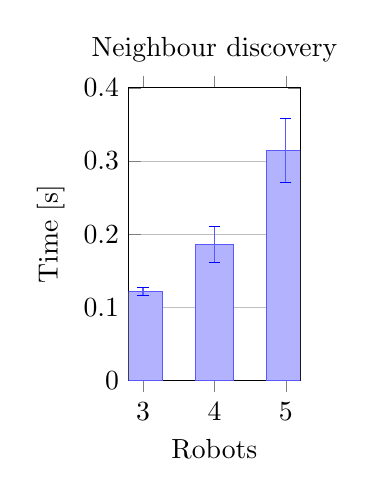
\begin{tikzpicture}
\begin{axis}[ybar,bar width=14pt,width=0.31\linewidth,height=5.3cm,symbolic x coords={3,4,5},xtick=data,ymin=0,ymax=0.40,ylabel={Time [s]},xlabel={Robots},title={Neighbour discovery},ymajorgrids=true]
\addplot+[draw=blue!65,fill=blue!30,error bars/.cd,y dir=both,y explicit] coordinates {(3,0.1218) +- (0,0.0055) (4,0.1861) +- (0,0.0248) (5,0.3144) +- (0,0.0432)};
\end{axis}
\end{tikzpicture}%
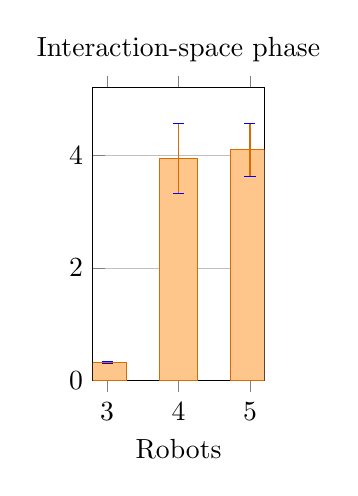
\begin{tikzpicture}
\begin{axis}[ybar,bar width=14pt,width=0.31\linewidth,height=5.3cm,symbolic x coords={3,4,5},xtick=data,ymin=0,ymax=5.2,xlabel={Robots},title={Interaction-space phase},ymajorgrids=true]
\addplot+[draw=orange!85!black,fill=orange!45,error bars/.cd,y dir=both,y explicit] coordinates {(3,0.3206) +- (0,0.0122) (4,3.9471) +- (0,0.6176) (5,4.0983) +- (0,0.4713)};
\end{axis}
\end{tikzpicture}%
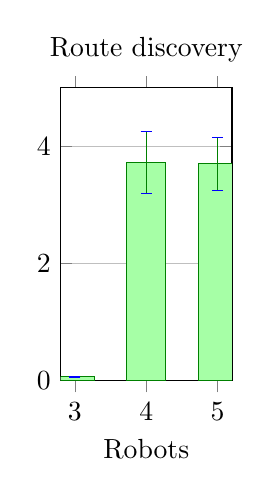
\begin{tikzpicture}
\begin{axis}[ybar,bar width=14pt,width=0.31\linewidth,height=5.3cm,symbolic x coords={3,4,5},xtick=data,ymin=0,ymax=5.0,xlabel={Robots},title={Route discovery},ymajorgrids=true]
\addplot+[draw=green!50!black,fill=green!35,error bars/.cd,y dir=both,y explicit] coordinates {(3,0.0643) +- (0,0.0136) (4,3.7260) +- (0,0.5342) (5,3.7021) +- (0,0.4472)};
\end{axis}
\end{tikzpicture}
